\chapter{Обобщение метода для неопределённостей}\label{ch:ch4}
\section{Мультипликативная мягкая неопределённость}\label{sec:ch4/sect1}

В этом подразделе мы рассмотрим случай, когда неопределённости ограничены следующим образом:
%
\begin{equation}
	\label{eq:part2_nu_uncertainty}
	{F}_i\T{F}_i\leq \nu_i {I}, \ \ i=1,2,3.
\end{equation}
%
Мы можем предложить условия на изменение коэффициента регулятора и наблюдателя, которые гарантируют устойчивость при любом допустимом значении ${F}_i$ для заданного радиуса неопределённости $\nu$:
\begin{theorem}\label{thm:part2_LMI_2}
	Система (\ref{eq:part2_system}) асимптотически стабильна для всех матриц
	$\Delta {A}_n={M}_1{F}_1{N}_1$, 
	$\Delta {B}= {M}_2{F}_2{N}_2$, 
	$\Delta {C} = {M}_3{F}_3{N}_3$
	где
	${F}_i\T{F}_i\leq \nu_i {I}$ для $i=1,2,3$
	если существуют такие позитивно-определённые матрицы ${Q}_1$, ${P}_2$и позитивные скаляры
	$\gamma_1>0$, $\gamma_2>0$, $\gamma_3>0$, $\bar{\mu}_1>0$, $\bar{\mu}_2>0$, $\bar{\mu}_3>0$, и $\epsilon_1 > 0$ такие, чтобы следующие линейные матричные неравенства выполнялись:
	%
	\begin{equation}
		\label{eq:thm4_final_LMI}
		\begin{bmatrix}
			{\Lambda}_1 & 0 & {M}_1 & {M}_2&0 & {Q}_1{N}_1\T & {\Lambda}_3 &{\Lambda}_4 & {B}\hat{{K}}_z & 0\\
			* & {\Lambda}_2 & {P}_2{M}_1 & {P}_2{M}_2 & \hat{{L}}_z{M}_3& 0& 0&0&0&{I} \\
			* & * & -\gamma_1{I} & 0&0&0&0&0&0&0\\
			* & * &*  & -\gamma_2{I}&0&0&0&0&0&0\\
			*& * & * &*  & -\gamma_3{I}&0&0&0&0&0\\
			* &* & * & * & *&-\bar{\mu}_1{I}&0&0&0&0\\
			* & * & * &*& *&*&-\bar{\mu}_2{I}& 0&{N}_2\hat{{K}}_z&0\\
			*&*&* &* & * & * & *&-\bar{\mu}_3{I}&0&0\\
			* & * & *&*&* & *&*&*&-\frac{1}{\epsilon_1}{Q}_1&0\\
			* & * & * & *&*&*&*&*&*&-\epsilon_1{Q}_1\\
		\end{bmatrix}<0,
	\end{equation}
	%
	где
	%
	\begin{align}
		{\Lambda}_3&=\hat{{K}}_z\T{N}_2\T,\\ {\Lambda}_4&={Q}_1{N}\T{N}_3\T,
	\end{align}
	%
	и ${\Lambda}_1$, ${\Lambda}_2$ определены в \eqref{eq:Lambda_1} и \eqref{eq:Lambda_2}. 
\end{theorem}
\begin{proof}
	Доказательство этой теоремы мы начинаем аналогично доказательству Теоремы \ref{thm:part2_LMI_1}, шаги, представленные уравнениями \eqref{eq:thm3_Lyapunov_candidat}-\eqref{eq:eta_3_thm3}, те же самые. Отсюда, используя \eqref{eq:part2_nu_uncertainty}, мы получаем:
	\begin{align}
		\label{eq:eta1_bound}
		\eta_1\T\eta_1 &\leq \chi\T \begin{bmatrix}
			{N}_1\T \\ 0  
		\end{bmatrix}\nu_1\begin{bmatrix}
			{N}_1 \ \ 0  
		\end{bmatrix} \chi,
		\\
		\eta_2\T\eta_2 &\leq \chi\T \begin{bmatrix}
			{K}_z\T{N}_2 \\ -{K}_z\T{N}_2\T  
		\end{bmatrix}\nu_2\begin{bmatrix}
			{N}_2{K}_z & -{N}_2{K}_z
		\end{bmatrix} \chi,
		\\
		\eta_3\T\eta_3 &\leq \chi\T \begin{bmatrix}
			-{N}\T{N}_3\T \\ 0  
		\end{bmatrix}\nu_3\begin{bmatrix}
			-{N}{N}_3 \ \ 0  
		\end{bmatrix} \chi.
	\end{align}
	%
	Используя S--процедуру из Леммы \ref{lemma:S_procedure} для включения вышеуказанных условий и обозначая $\bar{\mu}_i=\frac{1}{\mu_i}$, получаем:
	\begin{multline}
		\begin{bmatrix}
			{\Theta}_1 & -{P}_1{B}{K}_z & {P}_1{M}_1 & {P}_1{M}_2 &0 \\
			* &    {\Theta}_2 & {P}_2{M}_1 & {P}_2{M}_2 & {P}_2{L}_z{M}_3\\
			* & * & 0 & 0&0\\
			* & * & * & 0&0 \\
			* & * & * & *&0
		\end{bmatrix} + \\
		+ \begin{bmatrix}
			\mathcal{X}_{\mu}& -\mu_2{K}_z\T{N}_2\T{N}_2{K}_z &0 &0 & 0\\
			*&\mu_2{K}_z\T{N}_2\T{N}_2{K}_z&0&0&0\\
			*&*&-\gamma_1{I}&0&0\\
			*&*&*&-\gamma_2{I}&0\\
			*&*&*&*&-\gamma_3{I}\\
		\end{bmatrix} 
		<0,
	\end{multline}
	где
	%
	\begin{equation}
		\mathcal{X}_{\mu}=\mu_1{N}_1\T{N}_1 +\mu_2{K}_z\T{N}_2\T{N}_2{K}_z+\mu_3{N}\T{N}_3\T{N}_3{N},
	\end{equation}
	и $\mu_i=\gamma_i\nu_i$ для $i=1,2,3$.
	
Перепишем предыдущее неравенство как:
	\begin{multline}
		\label{eq:thm4_before_1Schur}
	\begin{bmatrix}
		{\Theta}_1 + \mathcal{X}_{S} & -{P}_1{B}{K}_z -\mu_2{K}_z\T{N}_2\T{N}_2{K}_z & {P}_1{M}_1 & {P}_1{M}_2 &0 \\
		* &    {\Theta}_2 + \mu_2{K}_z\T{N}_2\T{N}_2{K}_z & {P}_2{M}_1 & {P}_2{M}_2 & {P}_2{L}_z{M}_3\\
		* & * & -\gamma_1{I} & 0&0\\
		* & * & * & -\gamma_2{I}&0 \\
		* & * & * & *&-\gamma_3{I}
	\end{bmatrix} + \\
	+ \begin{bmatrix}
		N_1\T \\ 0 \\0\\0\\0
	\end{bmatrix} \mu_1
	\begin{bmatrix}
		N_1 & 0 & 0 & 0&0
	\end{bmatrix}
	<0,
\end{multline}
	где
%
\begin{equation}
	\mathcal{X}_{S}=\mu_2{K}_z\T{N}_2\T{N}_2{K}_z+\mu_3{N}\T{N}_3\T{N}_3{N}.
\end{equation}
Используя дополнение Шура из Леммы \ref{lemma:Schur}:
	\begin{equation}
	\label{eq:thm4_after_1Schur}
	\begin{bmatrix}
		{\Theta}_1 + \mathcal{X}_{S} & -{P}_1{B}{K}_z -\mu_2{K}_z\T{N}_2\T{N}_2{K}_z & {P}_1{M}_1 & {P}_1{M}_2 &0 & N_1\T\\
		* &    {\Theta}_2 + \mu_2{K}_z\T{N}_2\T{N}_2{K}_z & {P}_2{M}_1 & {P}_2{M}_2 & {P}_2{L}_z{M}_3 &0\\
		* & * & -\gamma_1{I} & 0&0&0\\
		* & * & * & -\gamma_2{I}&0&0 \\
		* & * & * & *&-\gamma_3{I}&0 \\
			* & * & * & *& *& -\bar{\mu}_1{I}
	\end{bmatrix}
	<0.
\end{equation}
	%
Повторяем шаги \eqref{eq:thm4_before_1Schur}--\eqref{eq:thm4_after_1Schur} два раза для устранения билинейности в переменных:
	\begin{equation}
		\label{eq:thm4_after_Schur}
		\begin{bmatrix}
			{\Theta}_1 & -{P}_1{B}{K}_z & {P}_1{M}_1 & {P}_1{M}_2 & 0 & {N}_1\T & {K}_z\T{N}_2\T & {N}\T{N}_3\T 
			\\
			* & {\Theta}_2 & {P}_2{M}_1 & {P}_2{M}_2 & {P}_2{L}_z{M}_3&0& -{K}_z\T{N}_2\T& 0\\
			* & * & -\gamma_1{I} & 0&0&0&0&0\\
			* & * & * & -\gamma_2{I}&0&0&0&0\\
			* & * & * & *&-\gamma_3{I}&0&0&0\\
			* & * & * & *&*&-\bar{\mu}_1{I}&0&0\\
			* & * & * & *&*&*&-\bar{\mu}_2{I}&0\\
			*&* & * & * & *&*&*&-\bar{\mu}_3{I}\\
		\end{bmatrix}<0.
	\end{equation}
	%
Умножаем справа и слева \eqref{eq:thm4_after_Schur} на $\text{diag}({Q}_1, {I})$, где ${Q}_1 = {P}_1^{-1}$:
%
\begin{equation}
	\label{eq:thm4_before_Young}
	\begin{bmatrix}
		{\Omega}_1 & -{B}{K}_z & {M}_1 & {M}_2 & 0& {Q}_1{N}_1\T & {Q}_1{K}_z\T{N}_2\T & {Q}_1 {N}\T{N}_3\T 
		\\
		* & {\Theta}_2 & {P}_2{M}_1 & {P}_2{M}_2 & {P}_2{L}_z{M}_3 & 0 & -{K}_z\T{N}_2\T & 0\\
		* & * & -\gamma_1{I} & 0&0&0&0&0\\
		* & * & * & -\gamma_2{I}&0&0&0&0\\
		* & * & * & *&-\gamma_3{I}&0&0&0\\
		* & * & * & *&*&-\bar{\mu}_1{I}&0&0\\
		* & * & * & *&*&*&-\bar{\mu}_2{I}&0\\
		*&* & * & * & *&*&*&-\bar{\mu}_3{I}
	\end{bmatrix}<0,
\end{equation}

Повторяя шаги \eqref{eq:thm3_before_Young_2}--\eqref{eq:after_Young_2}, 
используем Леммы \ref{lemma:Young} и \ref{lemma:Schur}, получаем:
\begin{equation}
	\label{eq:thm4_final_LMI_var}
	\begin{bmatrix}
		\mathcal{K}_{11} & \mathcal{K}_{12} \\
		* & \mathcal{K}_{22}
	\end{bmatrix}<0,
\end{equation}
где
\begin{equation}
	\mathcal{K}_{11}= \begin{bmatrix}
		{\Lambda}_1 & 0 & {M}_1 & {M}_2&0  \\
		* & {\Lambda}_2 & {P}_2{M}_1 & {P}_2{M}_2 & \hat{{L}}_z{M}_3\\
		* & * & -\gamma_1{I} & 0&0\\
		* & * &*  & -\gamma_2{I} &0\\
		*& * & * &*  &-\gamma_3{I}\\
	\end{bmatrix},
\end{equation}
%
\begin{equation}
	\mathcal{K}_{12}= \begin{bmatrix}
		{Q}_1{N}_1\T & \hat{{K}}_z\T{N}_2\T & {Q}_1 {N}\T{N}_3\T & {B}\hat{{K}}_z & 0\\
		0&0&0&0&I\\
		0&0& 0&0&0\\
		0&0&0& 0&0\\
		0&0&0&0&0\\
	\end{bmatrix},
\end{equation}
%
\begin{equation}
	\mathcal{K}_{22}=
	\begin{bmatrix}
		-\bar{\mu}_1{I}&0&0&0&0 \\
		*&-\bar{\mu}_2{I}& 0&{N}_2\hat{{K}}_z&0\\
		* & *&-\bar{\mu}_3{I}&0&0\\
		* & *&*&-\frac{1}{\epsilon_1}{Q}_1&0\\
		*&*&*&*&-\epsilon_1{Q}_1\\
	\end{bmatrix}.
\end{equation}%

Используем замену переменных $\hat{{K}}_z={K}_z{Q}_1$, $\hat{{L}}_z={P}_2{L}_z$, приходим к окончательному линейному матричному неравенству \eqref{eq:thm4_final_LMI}.
\end{proof}
В отличие от предыдущей задачи оптимизации, здесь не существует естественной формулировки целевой функции. Предлагается два варианта целевой функции:
\begin{align}
	\label{eq:cost_lin}
	J_\text{lin} &= \sum_{i=1}^{3}\left(\bar{\mu}_i+\gamma_i\right) \\ 
	\label{eq:cost_quad}
	J_\text{quad} & =  \sum_{i=1}^{3}\left((\bar{\mu}_i-\varpi)^2+(\gamma_i-\varpi)^2\right) + \varpi^2,
\end{align}
%
где $\varpi$ --- свободная переменная. Целью обеих целевых функций является максимизация $\nu_i$, которая достигается минимизацией либо $J_\text{lin}$, либо $J_\text{quad}$. Максимизируя $\nu_i$, мы достигаем устойчивости к большему набору неопределённых матриц $\Delta {A}_n$, $\Delta {B}$ и $\Delta {C}$.

Кроме того, может быть интересно ограничить набор неопределённых матриц, ограничив $\nu_i \leq 1$. Утверждение $\nu_i=\frac{1}{\bar{\mu_i}\gamma_i} \leq 1$ преобразуется в $\frac{1}{\bar{\mu}_i}\leq \gamma_i$, и, используя дополнение Шура, мы получаем линейное ограничение: 
%
\begin{equation}
	\label{eq:mu_gamma_limit}
	\begin{bmatrix}
		-\gamma_i & 1 \\
		1 & -\bar{\mu}_i
	\end{bmatrix}
	\leq 0. \end{equation}
%
Выбирая линейную целевую функцию и ограничивая $\nu_i$, задача оптимизации приобретает вид:
%
\begin{equation}
	\label{eq:thm4_OCP}
	\begin{aligned}
		& \underset{\bar{\mu}_i,\gamma_i,{Q}_1, {P}_2,\hat{{K}} , \hat{{L}} }{\text{минимизируя}}
		& &  \sum_{i=1}^{3}\left(\bar{\mu}_i+\gamma_i\right), \\
		& \text{при ограничениях}
		& & \begin{cases}
			{Q}_1>0, \ \
			{P}_2>0, \ \
			\bar{\mu}_i>0, \ \
			\gamma_i>0, \ \
			\text{для} \ \ i=1,2,3; \\
			\text{условия \eqref{eq:thm4_final_LMI}, \eqref{eq:mu_gamma_limit} }.
		\end{cases}
	\end{aligned}
\end{equation}
%
Данная задача оптимизации имеет параметр $\epsilon_1$ который мы можем найти решетчатым поиском.

Эту задачу можно рассматривать как обобщение и ослабление исходной задачи, рассмотренной в предыдущем подразделе. Вместо того чтобы искать управление, устойчивое к заданной неопределённости, мы пытаемся найти управление, устойчивое к наибольшей возможной неопределённости.

\section{Аддитивная неопределённость}\label{sec:ch4/sect2}

Рассмотрим следующую систему:
%
\begin{equation}
	\label{eq:part1_linear_dynamics}
	\begin{cases}
		\dot z=({A}_n+\Delta {A}_n)z + {A}_r\zeta + {B}u,\\
		y={C}{N}z+{C}{R}\zeta,
	\end{cases}
\end{equation}
%
где $z$ --- это динамические состояния, $\zeta = \text{const}$ --- статические состояния и $\Delta {A}_n$ представляет мультипликативную модель неопределённостей и имеет следующую структуру:
%
\begin{equation}
	\label{eq:part1_uncertainty}
	\Delta {A}_n={M}_1{F}_1{N}_1 \quad \text{и} \quad {F}_1\T{F}_1\leq \nu {I},
\end{equation}
%
где ${M_1} \in \mathbb{R}^{n_z \times d}$ и 
${N_1} \in \mathbb{R}^{d \times n_z}$ --- известные матрицы, ${F}_1$ --- неизвестная матрица ограниченная по норме и $\nu$ --- неизвестный радиус --- скаляр, определяющий лимит наложенный на норму ${F}_1$.

Следуя \cite{SAVIN2021} вводим наблюдатель Люенберга:
%
\begin{equation}
	\begin{bmatrix}
		\dot{\hat{z}} \\
		\dot{\hat{\zeta}}
	\end{bmatrix}=\begin{bmatrix}
		{A}_n & {A}_r \\
		0 & 0
	\end{bmatrix}
	\begin{bmatrix}
		\hat{z}\\ \hat{\zeta}
	\end{bmatrix}
	+  \begin{bmatrix}
		{B}\\0
	\end{bmatrix}u + {L} \left( y-\begin{bmatrix}
		{C}{N} & {C}{R}
	\end{bmatrix} \begin{bmatrix}
		\hat{z}\\ \hat{\zeta}
	\end{bmatrix} \right),
\end{equation}
%
где ${L}$ --- коэффициент наблюдателя.

Определим ошибку оценки состояния как $e = [ (z-\hat{z})\T \ \ (\zeta-\hat{\zeta})\T ]\T$ и введём блочные матрицы:
${S} = \begin{bmatrix}
	{I} \\ 0
\end{bmatrix}$, 
${E}=[ {N} \ \ {R}]$, и 
$
{A}_c=    \begin{bmatrix}
	{A}_r  & {A}_{\rho} \\
	0  & 0
\end{bmatrix}.
$

Записываем ошибку наблюдателя динамики:
%
\begin{equation}
	\label{eq:part1_error_dynamics}
	\dot e= ({A}_e-{L}{C}{E})e +{S}\Delta {A}_n z.
\end{equation}
%
Вводим закон управления:
%
\begin{equation}
	u={K}_z \hat{z}+{K}_{\zeta} \hat{\zeta},
\end{equation}
%
и определяем ${K}=\begin{bmatrix}
	{K}_z & {K}_{\zeta}
\end{bmatrix}$, записываем динамическую систему с обратной связью:
%
\begin{equation}
	\label{eq:part1_active_dynamics}
	\dot{z}=({A}_n+\Delta {A}_n +{B}{K}_z)z-{B}{K}e+({A}_r+{B}{K}_{\zeta})\zeta.
\end{equation}
%
Коэффициент регулятора ${K}_{\zeta}$ может быть выбран как:
%
\begin{equation}
	\label{eq:part1_static_control}
	{K}_{\zeta}=-{B}^{\dagger}{A}_r.
\end{equation}
%
Пока столбцы ${A}_r$ лежат в подпространстве столбцов ${B}$ и существует точная оценка состояния, данный закон управления сводит на нет эффект $\zeta$ на динамику. В данном случае, отмечая что ${K}_z={K}{S}$,  мы можем представить ошибку наблюдателя и динамику робота как систему уравнений:
%
\begin{equation}
	\label{eq:part1_system}
	\begin{bmatrix}
		\dot{z} \\ \dot{e}
	\end{bmatrix}=\begin{bmatrix}
		({A}_n+\Delta {A}_n +{B}{K}{S}) & {B}{K} \\
		{S} \Delta {A}_n & ({A}_e-{L}{C}{E})        \end{bmatrix}\begin{bmatrix}
		z \\ e
	\end{bmatrix}.
\end{equation}

Рассмотрим проблему нахождения таких коэффициентов регулятора и наблюдателя, которые будут давать устойчивую систему для всех допустимых значений $\Delta {A}_n$.

\subsection{Единичная неопределённость}\label{sec:ch4/sect2/sub1}

Начнём с рассмотрения случая, когда неопределённость строго ограничена неравенством ${F}_1\T{F}_1\leq {I}$, которое мы называем единичной неопределённостью. В этом случае следующая теорема даёт нам достаточное условие устойчивости, которое может быть непосредственно использовано при проектировании регуляторов и коэффициентов усиления наблюдателей и представлено в виде линейного матричного неравенства с параметром.

\begin{theorem}\label{thm:part1_LMI_1}
	Система \eqref{eq:part1_system} асимптотически устойчива для всех матриц $\Delta {A}_n={M}_1{F}_1{N}_1$ с ${F}_1\T{F}_1\leq {I}$, если существуют положительно-определённые матрицы ${Q}_1>0$, ${P}_2>0$, матрицы $\hat{{K}}, \hat{{L}}$ и скаляры $\epsilon_1>0,\epsilon_2>0,\epsilon_3>0$ такие, что следующее линейное матричное неравенство выполнимо: 
	%
	\begin{equation}
		\label{eq:thm1_final_LMI_ab}
		\begin{bmatrix}    
			{\Psi}_1  & 0 & {\Xi} & 0 &  {P}_1{N}_1\T & {Q}_1{N}_1\T & 0 & 0 & 0\\
			* & {\Psi}_2 & 0 & {I} & 0 & 0 & {P}_2{S}{M}_1 & 0 & 0\\
			* & * &  -\frac{1}{\epsilon_1}{H} & 0 & 0 &0 & 0& 0 & 0\\
			* & * & * & -\epsilon_1{H} & 0 & 0 & 0 & 0 & 0 \\
			* & * & * & * & -\epsilon_2 {I} & 0 & 0 & 0 & 0 \\      
			* & * & * & * & *&  -2\alpha {I} & 0 & \beta {I} &0 \\
			* & * & * & * & *& * & -2\beta {I} & 0 & \alpha {I} \\
			* & * & * & * & *&*&* &-{I}&0\\
			* & * & * & * & *&*&*&* &-{I}
		\end{bmatrix} <0,
	\end{equation}
	%
	где
	%
	\begin{equation}
		\label{eq:H_Xi_variables}
		{H} = \begin{bmatrix}
			{Q}_1 & 0 \\
			0 & {I}
		\end{bmatrix}, \ \ 
		{\Xi} = \begin{bmatrix}
			{B}\hat{{K}} & {B}{K}_{\zeta} \end{bmatrix},
	\end{equation}
	%
	\begin{align}
		\label{eq:Psi_1}
		{\Psi}_1&={Q}_1{A}_n\T+{A}_n{Q}_1+{B}\hat{{K}}+\hat{{K}}\T{B}\T  +\epsilon_2{M}_1{M}_1\T, \\
		\label{eq:Psi_2}
		{\Psi}_2 &={A}_e\T{P}_2+{P}_2{A}_e-\hat{{L}}{CE}-{E}\T{C}\T\hat{{L}}\T,
	\end{align}
	%
	и коэффициенты регулятора и наблюдателя находятся как ${L}={P}^{-1}_2\hat{{L}}$
	и ${KS}=\hat{{K}}{Q}^{-1}_1$.  
\end{theorem}

Доказательство Теоремы \ref{thm:part1_LMI_1} приведено в \cite{scbib1}.

Используя Теорему \ref{thm:part1_LMI_1} и добавляя выпуклую целевую функцию, мы формулируем робастную конструкцию управления в виде полуопределённой программы:
%
\begin{equation}
	\label{eq:thm1_OCP}
	\begin{aligned}
		& \underset{\epsilon_2,\alpha,\beta, {Q}_1, {P}_2,\hat{{K}} , \hat{{L}} }{\text{минимизируя}}
		& & \operatorname{tr}({Q}_1\T{W}_z{Q}_1)+ \operatorname{tr}({P}_2\T{W}_e{P}_2)+ \operatorname{tr}(\hat{{K}}\T{W}_k\hat{{K}})+\operatorname{tr}(\hat{{L}}\T{W}_l\hat{{L}}), \\
		& \text{при ограничениях}
		& & \begin{cases}
			{Q}_1>0, \ \
			{P}_2>0, \ \
			\epsilon_2>0, \ \
			\alpha>0, \ \
			\beta>0, \\
			\text{условие \eqref{eq:thm1_final_LMI_ab} },
		\end{cases}
	\end{aligned}
\end{equation}
где ${W}_z, {W}_e, {W}_k$ и ${W}_l$ --- весовые матрицы.
 
\subsection{Мягкая неопределённость}\label{sec:ch4/sect2/sub2}

Пусть матрица неопределённости $\Delta {A}_n$ определяется как:
%
\begin{equation}
	\label{eq:nu_uncertainty}
	\Delta {A}_n={M}_1{F}_1{N}_1 \quad \text{и} \quad {F}_1\T{F}_1\leq \nu {I}.
\end{equation}
%
Мы можем предложить условия на усиление регулятора и наблюдателя, которые гарантируют устойчивость при любом допустимом значении ${F}_1$ для заданного радиуса неопределённости $\nu$:
%
\begin{theorem}\label{thm:part1_LMI_2}
	Система \eqref{eq:part1_system}
	асимптотически устойчива для любой $\Delta {A}_n =$${M}_1{F}_1{N}_1$ с ${F}_1\T{F}_1\leq \nu {I}$, если существуют положительно--определённые матрицы ${Q}_1>0$, ${P}_2>0$, матрицы $\hat{{K}}, \hat{{L}}$ и скаляр $\bar{\epsilon}>0$ такие, что следующее линейное матричное неравенство выполнимо: 
	%
	\begin{equation}
		\label{eq:thm2_final_LMI}
		\begin{bmatrix}    
			{\Upsilon}_1  & 0 & {\Xi} & 0 &  {Q}_1{N}_1\T & {M}_1 & 0\\
			* & {\Psi}_2 & 0 & {I} & 0 & 0 & {P}_2{S}{M}_1\\
			* & * &  -\frac{1}{\epsilon_1}{H} & 0 & 0 &0 & 0\\
			* & * & * & -\epsilon_1{H} & 0 & 0 & 0 \\
			* & * & * & * & -\frac{\bar{\epsilon}}{2}{I} & 0 & 0 \\       * & * & * & * & *&  -\bar{\epsilon}{I} & 0 \\
			* & * & * & * & *& * &  -\bar{\epsilon}{I}
		\end{bmatrix} <0,
	\end{equation}
	%
	где
	%
	\begin{equation}
		\label{eq:Upsilon_1}
		{\Upsilon}_1={Q}_1{A}_n\T+{A}_n{Q}_1+{B}\hat{{K}}+\hat{{K}}\T{B}\T.
	\end{equation}
	Матрицы ${\Psi}_2$, ${\Xi}$ те же, что и в уравнениях \eqref{eq:Psi_2}, \eqref{eq:H_Xi_variables},
	а коэффициенты регулятора и наблюдателя задаются ${L}={P}^{-1}_2\hat{{L}}$
	и ${KS}=\hat{{K}}{Q}^{-1}_1$.
\end{theorem}
В качестве целевой функции мы можем использовать минимизацию $\bar{\epsilon}$, что эквивалентно максимизации $\nu$, так как $\nu=\frac{1}{\bar{\epsilon}^2}$. Тогда задача оптимизации приобретает вид:
%
\begin{equation}
	\label{eq:thm5_OCP}
	\begin{aligned}
		& \underset{\bar{\epsilon},{Q}_1, {P}_2,\hat{{K}} , \hat{{L}} }{\text{минимизируя}}
		& &  \bar{\epsilon}, \\
		& \text{при ограничениях}
		& & \begin{cases}
			{Q}_1>0, \ \
			{P}_2>0, \ \
			\bar{\epsilon}>0, \\
			\text{условие \eqref{eq:thm2_final_LMI} }.
		\end{cases}
	\end{aligned}
\end{equation}

\begin{remark}
	\label{rm:nu_trick}
	Добавление условия $\bar{\epsilon}\geq 1$ к \eqref{eq:thm5_OCP} эквивалентно ограничению $\nu \leq 1$. Это полезно, если мы заинтересованы в решении задачи ${F}_1\T{F}_1 \leq {I}$, но эта задача невыполнима, и мы хотели бы знать наибольший радиус $\nu$, для которого задача может быть решена. Таким образом, двоичный вопрос «да или нет» о выполнимости исходной задачи сводится к непрерывному вопросу «насколько велика неопределённость, которую мы можем допустить».
\end{remark}

\section{Эксперименты}\label{sec:ch4/sect3}

\subsection{Параметры эксперимента}\label{sec:ch4/sect3/sub1}

В данном разделе сначала показываем, как предложенные методы могут быть использованы для поиска наибольшего структурированного набора мультипликативных неопределённостей, которые может выдержать робастный линейный регулятор. Такая задача имеет ряд практических приложений. Она может быть использована для определения того, достигла ли конструкция регулятора своих пределов с точки зрения неопределённостей, которые он должен переносить. Задача также может быть решена для определения того, насколько велик набор неопределённостей, которые могут быть допустимы для данного конкретного робота и его конкретной конфигурации, что облегчает соответствующий анализ.

Далее приведено сравнение графиков для систем только с мультипликативными неопределённостями и со смешанными.
\subsection{Результаты эксперимента}\label{sec:ch4/sect3/sub2}

\begin{figure}[ht]
	\centerfloat{
		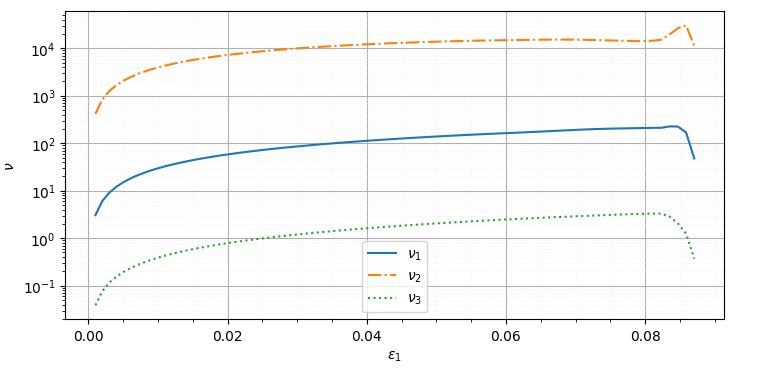
\includegraphics[scale=1.35]{images/mult_soft_nu_eps.JPG}
	}
	\caption{Верхняя граница радиусов неопределённости $\nu_i$, когда $\nu$ не ограничено для задачи \eqref{eq:thm4_OCP}; графики построены относительно значения свободного параметра $\epsilon_1$; вертикальная ось масштабирована логарифмически, обе оси без единиц.}\label{fig:mult_soft_nu}
\end{figure} 
Сначала, решаем оптимизационную задачу \eqref{eq:thm4_OCP} для различных значений $\epsilon_1$ для мягкой мультипликативной неопределённости. 
На Рисунке~\ref{fig:mult_soft_nu} показано, как наибольший радиус неопределённости $\nu$, который может выдержать регулятор, зависит от параметра $\epsilon_1$ (показан сплошной синей линией). График вогнутый, и появляется чётко определённое оптимальное решение. На этом же рисунке показан график, построенный при наложении условия \eqref{eq:mu_gamma_limit} (показано пунктирной красной линией). Видно, что наибольший радиус неопределённости ограничивается значением 1.

На Рисунке \ref{fig:mult_soft_less_than_unit} ограничим мягкую неопределённость 1.
\begin{figure}[ht]
	\centerfloat{
		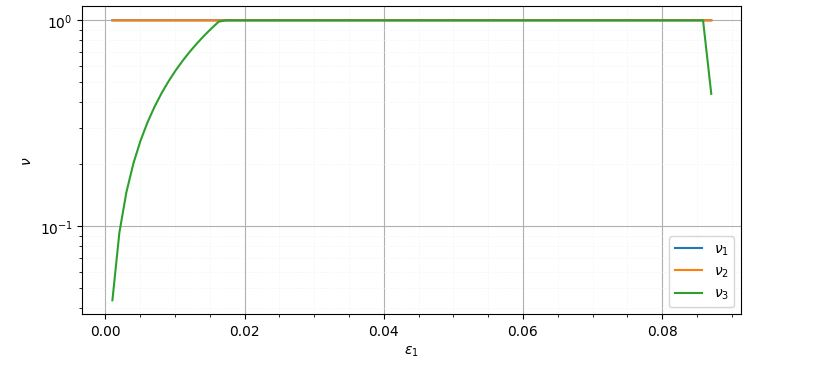
\includegraphics[scale=1.35]{images/mult_soft_less_than_unit.JPG}
	}
	\caption{Верхняя граница радиусов неопределённости $\nu_i$, когда $\nu$ не ограничено для задачи \eqref{eq:thm4_OCP} с целевой функцией \eqref{eq:cost_lin}; графики построены относительно значения свободного параметра $\epsilon_1$; вертикальная ось масштабирована логарифмически, обе оси без единиц.}\label{fig:mult_soft_less_than_unit}
\end{figure}


Затем решим оптимизационную задачу \eqref{eq:thm4_OCP} с квадратичной целевой функцией \eqref{eq:cost_lin}:

\begin{equation}
	\label{eq:thm5_OCP_qp}
	\begin{aligned}
		& \underset{\bar{\mu}_i,\gamma_i, \varpi, {Q}_1, {P}_2,\hat{{K}} , \hat{{L}} }{\text{минимизируя}}
		& &  \sum_{i=1}^{3}\left((\bar{\mu}_i-\varpi)^2+(\gamma_i-\varpi)^2\right) + \varpi^2, \\
		& \text{при ограничениях}
		& & \begin{cases}
			{Q}_1>0, \ \
			{P}_2>0, \ \
			\bar{\mu}_i>0, \ \
			\gamma_i>0, \ \
			\text{для} \ \ i=1,2,3; \\
			\text{условия \eqref{eq:thm4_final_LMI}, \eqref{eq:mu_gamma_limit} }.
		\end{cases}
	\end{aligned}
\end{equation} 

\begin{figure}[ht]
	\centerfloat{
		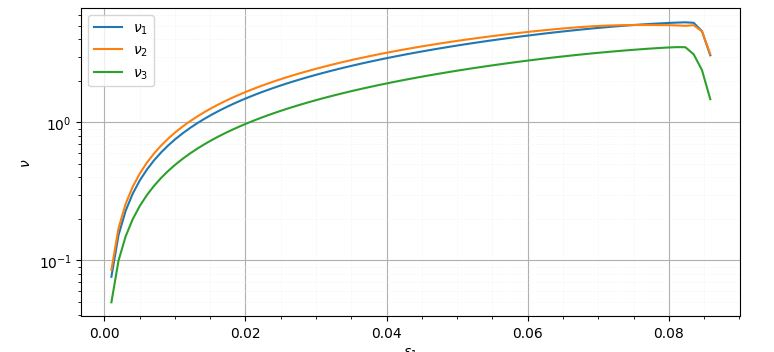
\includegraphics[scale=1.35]{images/mult_soft_nu_eps_qp.JPG}
	}
	\caption{Верхняя граница радиусов неопределённости $\nu_i$, когда $\nu$ не ограничено для задачи \eqref{eq:thm5_OCP}; графики построены относительно значения свободного параметра $\epsilon_1$; вертикальная ось масштабирована логарифмически, обе оси без единиц.}\label{fig:mult_soft_nu_eps_qp}
\end{figure}


\begin{figure}[ht]
	\centerfloat{
		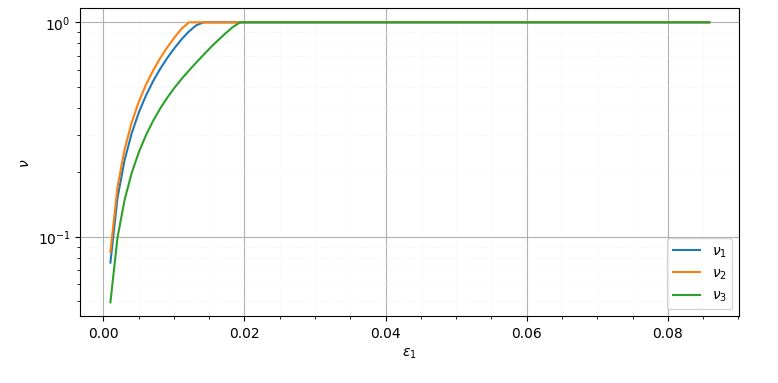
\includegraphics[scale=1.35]{images/mult_soft_less_than_unit_qp.JPG}
	}
	\caption{Верхняя граница радиусов неопределённости $\nu_i$, когда $\nu$ ограничено для задачи \eqref{eq:thm5_OCP}; графики построены относительно значения свободного параметра $\epsilon_1$; вертикальная ось масштабирована логарифмически, обе оси без единиц.}\label{fig:mult_soft_leq_qp}
\end{figure}

На Рисунке \ref{fig:mult_soft_leq_qp} показана зависимость радиусов неопределённости от параметра $\epsilon_1$.
